\documentclass[a4paper,12pt]{article}

\usepackage{tikz}    % diagramas
\usepackage{amsmath} % align
\usepackage{amssymb} % mathbb, varnothing
\usepackage{xspace}

\usetikzlibrary{arrows.meta} % para mudar o tamanho das cabeças das setas

\newcommand{\seta}{\draw[-{>[scale=2,width=2]},line width=0.5pt]}
\newcommand{\sums}{\texttt{SUMS}\xspace}
\newcommand{\sat}{\texttt{SAT}\xspace}
\newcommand{\np}{\textbf{NP}\xspace}

\title{Projeto 1: \sat em {Z3}}
\author{João Miguel Faria \and Rui Breda Perdigoto}
\date{\today}

\begin{document}
\maketitle

\section{Sudoku}
%\subsection{Classic Sudoku}

\subsection{Descrição do problema}
Este exercício do projeto consistiu na modelação e redução do problema do
sudoku para \sat. Este problema consiste no seguinte: dado um tabuleiro inicial
9x9, preencher todas as células do tabuleiro com números de 1 a 9 tal que
nenhum número se repita na mesma linha, coluna e região (quadrado 3x3).

\subsection{Símbolos Proposicionais}
Uma abordagem à resolução deste problema através do SAT-solver z3 implica que
este seja descrito como fórmulas de símbolos proposicionais em CNF (Conjunctive
Normal Form). Fórmulas estas que serão testadas face diversas atribuições aos
símbolos proposicionais.

Uma vez que se pretende explicitar que nenhuma célula pode ter um número já
presente na mesma linha, coluna e região, o número de símbolos proposicionais
não poderia ser inferior a $9\times9$. Como o domínio onde trabalhamos é
booleano, cada número que as células podem ter terá que ser um símbolo
proposicional, com o valor verdadeiro se o número se encontra na célula e falso
coso contrário.
 
Portanto, haverá no total um símbolo por cada célula e por cada número
possível, resultando em 9$\times$9$\times$9 símbolos. Assim, os símbolos terão
a forma \texttt{p\_i\_j\_n}\_, $0\leq i, j \leq 8$
e $1 \leq n \leq$ 9 com $i$ e $j$ os índices da célula no tabuleiro e n um
número possível de 1 a 9.

\subsection{Condições e restrições}
Estabelecidos os símbolos proposicionais, é necessário descrever o problema em
termos de condições e restrições ás quais este será sujeito.  Como foi referido
anteriormente, cada célula necessita de ter um e um só número. Esta condição
pode ser dividida em duas:
\begin{itemize}
     \item Cada célula tem pelo menos um número, ou seja, os símbolos da
        respetiva célula e dos diversos números não podem ser todos
        simultaneamente falsos.
        \begin{align}
        \bigwedge_{0\leq i,j < 9}
           \bigvee_{1\leq n \leq 9} p_{i,j,n}
        \end{align}
     
     \item Cada célula tem no máximo um número. A presença desta condição é justificada pelo facto de, se houver mais do que um número por célula, os restantes números da linha, coluna e região serão influenciados.
        \begin{align}
        \bigwedge_{0\leq i,j < 9}
         \bigwedge_{1\leq k < m < 9} \lnot p_{i,j,k}
           \bigvee \lnot p_{i,j,k}
        \end{align}
     
      \item Feitas as condições para as células, é necessário implementar as
         restrições que ditam as regras do puzzle.  As seguintes restrições
         indicam que uma linha e uma coluna não podem ter um número repetido,
         com a única diferença entre as duas ser os índices de p.
         \begin{align}
         \bigwedge_{0\leq i < 9} \bigwedge_{1\leq k \leq 9} \bigwedge_{0\leq j < m
         < 9} \lnot p_{i,j,k}
         \bigvee \lnot p_{i,j,k}
         \end{align}

         \begin{align}
         \bigwedge_{0\leq i,j < 9} \bigwedge_{1\leq k < m < 9} \lnot p_{i,j,k}
         \bigvee \lnot p_{i,j,k}
         \end{align}
\end{itemize}

\subsection{Variantes}

\section{\sums}
\subsection{Descrição do problema}
Sudoku mas com cenas extra

\subsection{Observações sobre a Complexidade}
Para qualquer um dos problemas, há três complexidades que nos interessam: a
original, a final e a da redução. 
\sums está claramente em \np.
Aqui, há duas
No Sudoku este problema não surge, mas aqui sim, porque há duas reduções
óbvias, ambas exponenciais:
\begin{itemize}
   \item num extremo, temos $p_r$ para cada $r\in R$ Neste caso, encontrar
      $S=\{r_{i_1},\cdots r_{i_j}\}$ é o mesmo que encontrar uma valoração
      Mas definir as restrições é equivalente a encontrar uma valoração

   \item Noutro, temos $p_S$ para cada $S\subseteq R$, em que $p_S=\top$ sse
      $S$ satisfaz o pedido
      Aqui a explosão exponencial acontece logo no número de proposições, a
      resolução do SAT só aparece depois de resolver o problema
\end{itemize}

Surge então a ideia de fazer $p_{u,r}$ em que $u\in R$ é o último dígito e
$r\in [0,t]\cap\mathbb N$ representa quanto falta para chegarmos a $t$.

Temos que ter cuidado se a notação é $p_{4,3}$ ou $p_{4,7}$ ou algo do género

\begin{figure}%[h]
\begin{minipage}{0.4\textwidth}
   \centering
   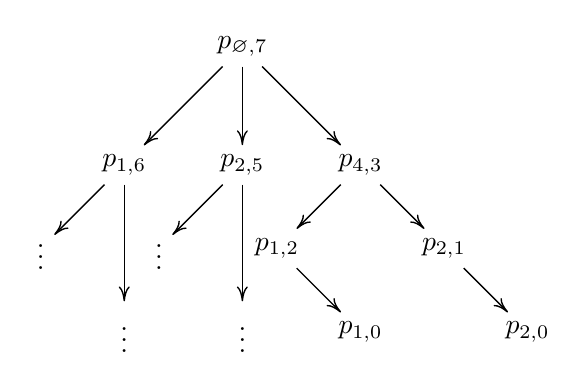
\begin{tikzpicture}[node distance=1.5cm]
      % níveis 0 e 1
      \node(p43)                    {$p_{4,3}$};
      \node(p25)  [left of=p43]     {$p_{2,5}$};
      \node(p16)  [left of=p25]     {$p_{1,6}$};
      \node(p07)  [above of=p25] {$p_{\varnothing,7}$};

      \seta(p07) -- (p16);
      \seta(p07) -- (p25);
      \seta(p07) -- (p43);

      % nível 2
      \node(x1)  [below left of=p16]   {$\vdots$};
      \node(x2)  [below right of=x1]   {$\vdots$};
      \node(x3)  [right of=x1]         {$\vdots$};
      \node(x4)  [below right of=x3]   {$\vdots$};
      \node(p12) [below left of=p43]   {$p_{1,2}$};
      \node(p21) [below right of=p43]  {$p_{2,1}$};

      \seta(p16) -- (x1);
      \seta(p16) -- (x2);
      \seta(p25) -- (x3);
      \seta(p25) -- (x4);
      \seta(p43) -- (p12);
      \seta(p43) -- (p21);

      % nível 3
      \node(p10) [below right of=p12]  {$p_{1,0}$};
      \node(p20) [below right of=p21]  {$p_{2,0}$};

      \seta(p12) -- (p10);
      \seta(p21) -- (p20);
   \end{tikzpicture}
\end{minipage}
\hfill
\begin{minipage}{0.4\textwidth}
\end{minipage}
\end{figure}
\end{document}
